\documentclass[tikz]{standalone}

\pagestyle{empty}


\usepackage{amsmath}
\usepackage{tikz}
\usepackage{graphicx}
\usetikzlibrary{positioning,calc,fit,decorations.pathreplacing,arrows,positioning,backgrounds}

% Font settings:
\renewcommand{\familydefault}{\sfdefault}
\usepackage{pxfonts}
\newcommand{\figf}{\sffamily\bfseries\small} %Defines the font used for the labelling of figure panels.


% Color settings:
%\definecolor{hivc}{cmyk}{0,0.80,0.83,0.13}                %\definecolor{hivc}{HTML}{DE2D26}
\definecolor{hivc}{RGB}{24,116,205}
\definecolor{selfc}{cmyk}{0,0,0,0.6}                      %\colorlet{selfc}{gray!80!white}
\definecolor{Rblue}{RGB}{100,149,237}


\begin{document}
\scriptsize

\begin{tikzpicture}[anchor=north west]

	\clip (0,0) rectangle +(18,-12);
	\begin{scope}[yshift=0cm]
		\node[anchor = north west] at (0.2,0) {
			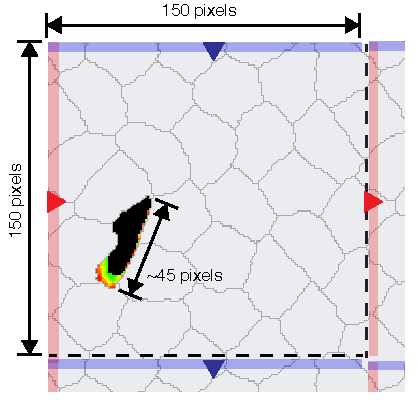
\includegraphics{../cartoons/skin-setup.pdf}
		};
	
		\node[anchor = north west] at (0,0) {\figf A};		
	\end{scope}

	\begin{scope}[xshift=7.7cm]


		\begin{scope}
			\node[anchor = north, align = center] at (3.15,-0.35){
				$\lambda$\textsubscript{act} = 1000:
			};
			\node[anchor = north west] at (1.5,-0.7) { "stop" };
			\node[anchor = north west] at (3.8,-0.7) { "go" };
			\begin{scope}[xshift=1cm, yshift=-1.1cm]
				\clip (0,0) rectangle +(2,-2);
				\node[anchor = north west, scale = 0.4 ] at (-1.3,0.5) {
					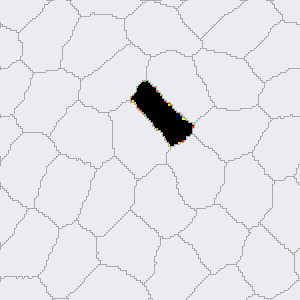
\includegraphics{../example-img/M30L1000-stop-t0.png}
				};
			\end{scope}

			\begin{scope}[xshift=3.2cm, yshift=-1.1cm]
				\clip (0,0) rectangle +(2,-2);
		
				\node[anchor = north west, scale = 0.4 ] at (-1.3,0.5) {
					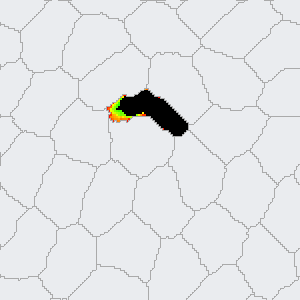
\includegraphics{../example-img/M30L1000-go-t15.png}
				};
			\end{scope}
		\end{scope}
	
		\begin{scope}[xshift=4.8cm]
			\node[anchor = north, align = center] at (3.15,-0.35){
				$\lambda$\textsubscript{act} = 2000:\\
				protrusion splitting
			};

			\begin{scope}[xshift=1cm, yshift=-1.1cm]
				\clip (0,0) rectangle +(2,-2);
				\node[anchor = north west, scale = 0.4 ] at (0,0.7) {
					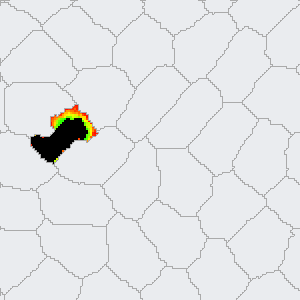
\includegraphics{../example-img/M30L2000-t0.png}
				};
			\end{scope}

			\begin{scope}[xshift=3.2cm, yshift=-1.1cm]
				\clip (0,0) rectangle +(2,-2);
		
				\node[anchor = north west, scale = 0.4 ] at (0,0.7) {
					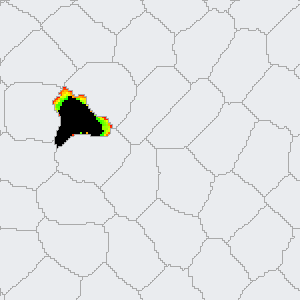
\includegraphics{../example-img/M30L2000-t10.png}
				};
			\end{scope}
		\end{scope}
	
	
		\begin{scope}[yshift=-3.65cm]
			\node[anchor = north, align = center] at (3.15,-0.35) {
				$\lambda$\textsubscript{act} = 300:\\
				protrusion splitting
			};

			\begin{scope}[xshift=1cm, yshift=-1.1cm]
				\clip (0,0) rectangle +(2,-2);
				\node[anchor = north west, scale = 0.4 ] at (0,2.1) {
					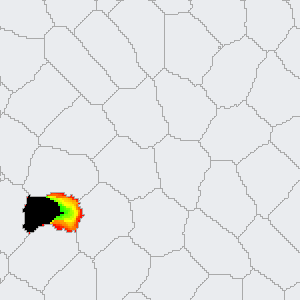
\includegraphics{../example-img/M100L300-t0.png}
				};
				%\draw[->] (1.05,-1.0) -- +(0.25,-0.05);
			\end{scope}

			\begin{scope}[xshift=3.2cm, yshift=-1.1cm]
				\clip (0,0) rectangle +(2,-2);
		
				\node[anchor = north west, scale = 0.4 ] at (0,2.1) {
					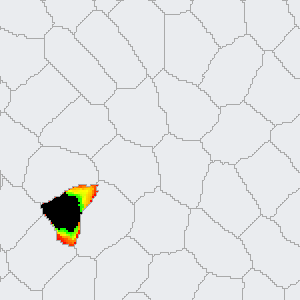
\includegraphics{../example-img/M100L300-t20.png}
				};
				%\draw[->] (0.95,-1.2) -- +(-0.05,-0.2);
			\end{scope}
		\end{scope}

		\begin{scope}[xshift=4.8cm,yshift=-3.65cm]
			\node[anchor = north, align = center] at (3.15,-0.35) {
				$\lambda$\textsubscript{act} = 1000:\\
				protrusion splitting
			};

			\begin{scope}[xshift=1cm, yshift=-1.1cm]
				\clip (0,0) rectangle +(2,-2);
				\node[anchor = north west, scale = 0.4 ] at (-0.5,1.5) {
					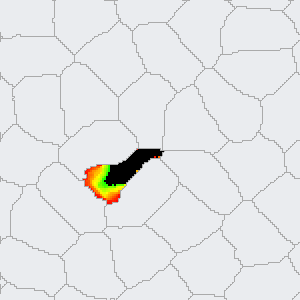
\includegraphics{../example-img/M100L1000-t40.png}
				};
				%\draw[->] (1.05,-1.0) -- +(0.25,-0.05);
			\end{scope}

			\begin{scope}[xshift=3.2cm, yshift=-1.1cm]
				\clip (0,0) rectangle +(2,-2);
		
				\node[anchor = north west, scale = 0.4 ] at (-0.5,1.5) {
					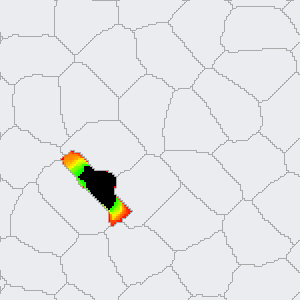
\includegraphics{../example-img/M100L1000-t65.png}
				};
				%\draw[->] (0.95,-1.2) -- +(-0.05,-0.2);
			\end{scope}
		\end{scope}


		%\node[anchor = north west, scale = 0.5 ] at (6,0) {
		%	\includegraphics{./img/skin-l1300-broad.png}
		%};
		\node[rotate = 90, anchor = north] at (0.5,-2.1) {maxact = 30:};	
		\node[rotate = 90, anchor = north] at (0.5,-5.75) {maxact = 100:};	
	
		\node[anchor = north west] at (0,0) {\figf B};	
		%\node[anchor = north west] at (0,-3.5){\figf C};		
	\end{scope}

	\begin{scope}[yshift=-7cm]
		\begin{scope}[xshift=0.1cm,yshift=-0.3cm]

			\node[anchor=north west] at (1,0.1) {stiff tissue:};

			\begin{scope}[xshift=1cm, yshift=-0.3cm]
				\clip (0,0) rectangle +(1.7,-1.7);
				\node[anchor = north west, scale = 0.3 ] at (-0.6,0.75) {
					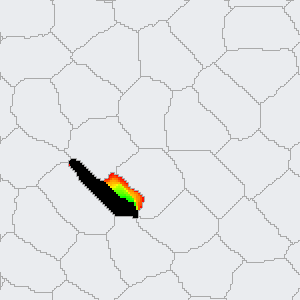
\includegraphics{../example-img/M100L1000-t146.png}
				};
				%\draw[->] (1.05,-1.0) -- +(0.25,-0.05);
			\end{scope}

			\begin{scope}[xshift=2.8cm, yshift=-0.3cm]
				\clip (0,0) rectangle +(1.7,-1.7);
		
				\node[anchor = north west, scale = 0.3 ] at (-0.6,0.75) {
					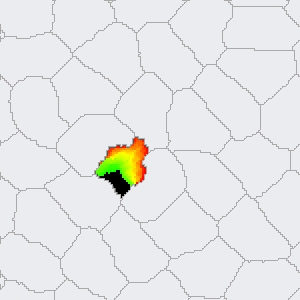
\includegraphics{../example-img/M100L1000-t167.png}
				};
				%\draw[->] (0.95,-1.2) -- +(-0.05,-0.2);
			\end{scope}
		
			\begin{scope}[xshift=4.6cm, yshift=-0.3cm]
				\clip (0,0) rectangle +(1.7,-1.7);
		
				\node[anchor = north west, scale = 0.3 ] at (-0.6,0.75) {
					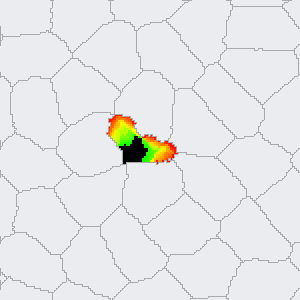
\includegraphics{../example-img/M100L1000-t187.png}
				};
				%\draw[->] (0.95,-1.2) -- +(-0.05,-0.2);
			\end{scope}
		\end{scope}
	
		\begin{scope}[xshift=0.1cm,yshift=-2.5cm]

			\node[anchor=north west] at (1,0.1) {deformable tissue:};

			\begin{scope}[xshift=1cm, yshift=-0.3cm]
				\clip (0,0) rectangle +(1.7,-1.7);
				\node[anchor = north west, scale = 0.3 ] at (-1.5,0.15) {
					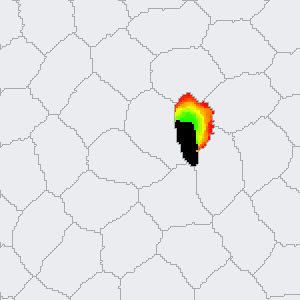
\includegraphics{../example-img/deformable-M100L1000-t67.png}
				};
				%\draw[->] (1.05,-1.0) -- +(0.25,-0.05);
			\end{scope}

			\begin{scope}[xshift=2.8cm, yshift=-0.3cm]
				\clip (0,0) rectangle +(1.7,-1.7);
		
				\node[anchor = north west, scale = 0.3 ] at (-1.5,0.15) {
					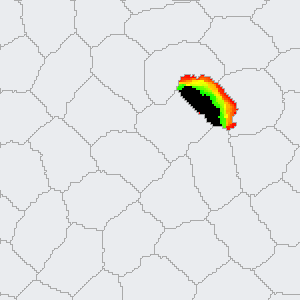
\includegraphics{../example-img/deformable-M100L1000-t97.png}
				};
				%\draw[->] (0.95,-1.2) -- +(-0.05,-0.2);
			\end{scope}
		
			\begin{scope}[xshift=4.6cm, yshift=-0.3cm]
				\clip (0,0) rectangle +(1.7,-1.7);
		
				\node[anchor = north west, scale = 0.3 ] at (-1.5,0.15) {
					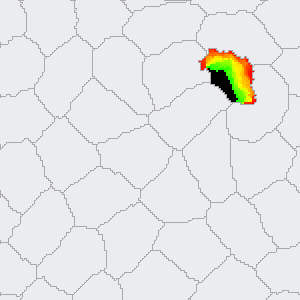
\includegraphics{../example-img/deformable-M100L1000-t127.png}
				};
				%\draw[->] (0.95,-1.2) -- +(-0.05,-0.2);
			\end{scope}
		\end{scope}

	
		\node[anchor = north west] at (0,0) {\figf C};	
	\end{scope}


	\begin{scope}[xshift = 6.9cm,yshift=-7cm]
		\node[anchor = north west] at (0,0) {
			\includegraphics{../plots/F5panelD.pdf}
		};
		\node[anchor = north west] at (0,0) {\figf D};		
	\end{scope}


\end{tikzpicture}




\end{document}